\chapter{Usability Testing}
\label{chap:usabilityTesting}
One of the project's goals is to create an interface which has a high degree of user friendliness. This coincides with that software projects  are usually tested against users before eventual release.\\
This chapter will describe the usability test conducted for the developed interface.

%How did we do the test
	%Who was where
	%The simularity of the questions
\section{Structure of the test}
The test was performed in Cassiopeias usability lab, shown on \autoref{fig:usabilitylab},  where a computer, in subject room one, was logged onto our website.
Each test person was lead into the test room and offered a cup of coffee, after which they were given a short briefing and asked to sign a consent form in which they agreed to that they were being filmed for research purposes.\\
After the introduction the test person was asked to perform a set of short assignments which were designed in such a way that they would try the complete set of implemented features in the system. 
When the test person had completed all the assignments,  he was given a set of follow-up questions about some of the ways that the test person used the system during the test.\\
During all completed tests it was the same person performing the role as instructor, as to not get biased test results.\\
The assignments as well as the introduction given to all participants can be found in appendix \vref{usabilityTestingAppendix}.\\
\\

\begin{figure}[!h]
	\centering
		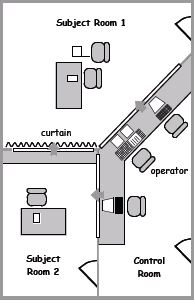
\includegraphics[width=0.40\textwidth]{images/usabilitylab.png}
	\caption{Usability Lab}
	\label{fig:usabilitylab}
\end{figure}

	%Picking the candidates
The usability test was performed with four test persons. Even though that number is not very high the actual number of people which will be using the advanced features of the system such as creating profiles will not be much higher when the system is deployed. One of the test persons, which job include daily leadership of a kindergarten, was before the test considered one of those who will actually work with the advanced features but during the follow-up questions it became clear that this might not be the case. The test can therefore be seen as a little biased as to having test persons without the appropriate level of technological knowledge. As this person might work with the system's advanced features in the future this person is viewed as a proper user and the other three as confirmation subjects. Two of these confirmation subjects work with children which has autism, every day and the last is an educated computer scientist as well as a parent to a child with autism. The latter person is considered to have a higher level of technological knowledge than the eventual users of the advanced features and was mainly used for confirming critical bugs and give suggestions for new features.\\
Upon eventual release all of the test persons would work with the non-advanced features, if not on a daily then on a weekly basis.

	%The old version
As the developed system at the time of the test was not in a state were it was stable enough to test on, an older version of the administrative interface was used during the test. The version which was used during the test can be collected from GitHub \citep{testBranch}.\\
\\
\section{Result of the test}
Table \ref{tab:Bugs/Errors} displays the errors or bugs, which was found during the usability test. They are described by a category, the error itself, its severity and lastly if it is corrected in the final version before hand-in.\\
They have been sorted by the severity of the error, and here we use three categories, critical, serious and cosmetic. Critical depicts an error which either makes a general task impossible or made the user stop altogether. Serious depicts an error which made the user stop for some time, or seemed to be unnecessarily distracting. Cosmetic depicts an error of low calibre, which even some of the users informed us was minor issues which did not affect the flow.\\
\\

%Result of the test
	%Bugs/Errors
		%Severity
\begin{table}[htbp]
	\centering
		\begin{tabularx}{\textwidth}{|X|l|l|}
			\hline
			Description & Severity & Corrected\\\hline\hline
			Pictograms - It is not possible to create new categories of Pictos & Critical &\\\hline
			Profile - Restrict QR editing to department manager & Critical &  \\\hline 
			DB Problem - Not possible for all pedagogues to fix Pictos for all department children & Critical & \\\hline
			Navigation - The site ''Profiles'' should link to each profile & Critical &\\\hline
			Missing - Unable to remove relations & Critical & \\\hline
			Profile Pic - Accept button is hard to find & Serious &\\\hline
			Profile Pic - Word ''change'' is misleading & Serious &\\\hline
			Navigation - ''Add'' and ''Make'' under Pics Manager is confusing & Serious & \\\hline
			Navigation - Language Support on navigation did not change to Danish & Serious & X\\\hline
			Missing - No Danish language support on the site ''Profiles''& Serious & X\\\hline
			Profile - Department should be a link, not editable & Serious & (X)\\\hline
			Profile - Links from Own Profile relations is missing & Serious & \\\hline
			Profile Pic - GIRAF Logo as Place holder is misleading  & Cosmetic & X\\\hline
			Profile Pic - Word ''Edit'' is not informative & Cosmetic &\\\hline
			DB Problem - Own Profile takes too long to load & Cosmetic &  \\\hline
			Navigation - ''Add Relation''  is before ''Create Profile'' & Cosmetic & X \\\hline
			Design - Standardize button names & Cosmetic & \\\hline
			Logout - Can navigate in system without session & Cosmetic & \\\hline
	\end{tabularx}
	\caption{Bugs/Errors Found Under Usability Testing}
	\label{tab:Bugs/Errors}
\end{table}

%What have we already fixed
Some of these errors was nearly immediately rectified, or had already been solved in the system which was up to date. These can be seen in table \ref{tab:Bugs/Errors} as ''X''. If the X, is marked with parentheses, it is because the problem have been partially solved.\\
\\
%What MUST be fixed
As mentioned before there is errors marked critical, as can be seen by the first 5 entries in the table. These are errors which must be fixed for the system to be able to use the implemented feature set, as listed in chapter \vref{chap:systemOverview}.\\
Next an explanation of the critical problems, and in short how they can be rectified.\\
\\
\textbf{Pictograms - It is not possible to create new categories of Pictos}\\
This error arose because the task of creating categories was not thought through. This is one feature which was overlooked, even after having had a meeting with the contact person, and showing the intended feature set.\\
Solving this error requires the creation of a minor tool which makes it possible to create and assign categories by a simple entry of a text string. For navigation purposes this tool should be under the Pics Manager category in the navigation menu.\\
\\
\textbf{Profile - Restrict QR editing to department manager}\\
After the first test person, it was made clear that the test person thought highly of the QR code, which they are given for the system. It is supposed to be as important as your house key, and should therefore not be something which can easily be changed.\\
To accommodate for this request the QR changer should not be available from the Own Profile site. Instead the procedure will be to contact the administrator of the system and have him generate a new key with the QR Manager tool and then send this out.\\
\\
\textbf{DB Problem - Not possible for all pedagogues to fix pictos for all department children}\\
This problem most likely erupted from a misunderstanding between the DB group, WASTELAND, and ourselves. The problem is that in order for a pedagogue to edit anything about a child in its department they need to have a relation between them. But this is not how the user intends to use the system. The relation should only be thought of as a responsibility link, and only adds the feature to change this child's profile data.\\
There is no easy way to rectify this problem from the admin projects side. This has to be fixed inside the database, because of its security mechanisms. For a solution to this it is suggested to look at the database project, WASTELAND \citep{wasteland}.\\
\\
\textbf{Navigation - The site ''Profiles'' should link to each profile}\\
This is simply a matter of a feature which has not yet been implemented. It is shown here as an error, because it is necessary for the system to be operated correctly.\\
It can be fixed by adding normal HTML anchor links to each name in the tables.\\
\\
\textbf{Missing - Unable to remove relations}\\
This is again a matter of a feature which have not yet been implemented.\\
This feature is thought to be usable only for the department manager and the administrator of the system and it should be used directly from each users profile. This means that the administrator or department manager, navigates to the user's profile, find the person he or she is related to and clicks the button to remove the relation.\\
\\
The rest of the errors is not of a nearly as urgent calibre, and will therefore not be discussed further in this report.\\

\section{New Features}
Instead the attention is turned to the possible extra features found during the test, both inspired by the way the users used the system, and their commentary afterwards.\\
\\

	%Features
\begin{table}[htbp]
	\centering
		\begin{tabular}{|l|}
			\hline
			Description\\\hline\hline
			Make the modal window customizable \\\hline
			Profile - Press enter to save change \\\hline
			Pics Manager Make - Add recording feature\\\hline
			Input forms - Automatic first letter uppercase for name and address\\\hline  
			Navigation - Add link to ''add relations'' and ''create profile'' in Profiles \\\hline  
			Pics Manager Make - Directly create picto for child from profile page \\\hline
			Pics Manager Make - Auto add ''inline-text'' to picto preview \\\hline
		\end{tabular}
	\caption{Features Found Under Usability Testing}
	\label{tab:NewFeature}
\end{table}	

%What could be added later - Maybe a refference to Future Work instead?
As seen from table \ref{tab:NewFeature} there is a few features which could improve the system. Some of the features which might be a bit hard to understand without having been on the development team is explained in detail in the following text.\\
\\
\textbf{Make the modal window customizable}\\
During this project a modal window was designed because of some issues with the bootstrap library. It seemed that the user sometimes found it confusing with the many cancel options which is offered for closing the modal window, even though it follows the way bootstrap displays their modal windows.\\
But also in the long run it could be useful to have the ability to customize the modal window with more than a title and a text.\\
\\
\textbf{Input forms - Automatic first letter upper case for name and address}\\
While watching the users work in the system, multiple times it was witnessed that they deleted a full text string because they entered the first letter of an address or a name in lower-case. therefore to save the user time, making each word in the address and name field automatically convert to upper-case since that is the custom with all names and addresses.\\
\\
\textbf{Navigation - Add link to ''add relations'' and ''create profile'' in Profiles}\\
Some of the users in the test meant that the most meaningful way to handle profiles, would be directly from the menu point ''Profiles'', and did not bother to look just below this menu point, where these options lay. This behaviour was seen in 3 out of 4 cases, and should therefore be considered.\\
It is a simple addition and does not hinder the system in any way. So if it even only helps a few people in the beginning of the learning of the system, this is feature worth having.\\
\\
\textbf{Pics Manager Make - Directly create Picto for child from profile page}\\
While watching the users work in the system, and also afterwards, when they were interviewed. We came to understand that some of the pedagogues, in our test case, 2 out of 3. Thought of the child as the central element in the system and therefore wanted to create everything out from the child.\\
This meant that when they had to add parents or pictograms to the child, they went to try and find the child's profile. therefore in order to accommodate this behaviour we should implement a feature which makes it possible to automatically relate a child and a Guardian as well as a child and a pictogram, when the action is started from that child's profile.\\
\\
\textbf{Pics Manager Make - Auto add ''inline-text'' to picto preview}\\
Some of the users did not quite understand what the inline-text field in the Pics Manager Make function meant, before we asked them. Which after they immediately understood what it was for, without us telling them. During the test, we even saw one of our test persons fill the field, and then delete the entry again.\\
If this was a result of the assignment regarding the use of pictograms did not specify that the inline-text field needed to be filled, or something else, we are not certain.\\
But a way to avoid this problem would be to simply add a JavaScript feature which automatically writes on top of the temporary display of the new pictogram.\\
\\
\\
The reader should now be as well informed of the structure and shortcomings of the GIRAF Admin system, as the developer group was. But in case the reader wants more information about the system, the reader should try to contact Ulrik Nyman, Associate Professor at Aalborg University and ask about the GIRAF Admin group of the summer semester, year 2013.\\
In the next chapter we draw conclusions about the system as a whole, and after that we make an evaluation of the process and the multi-project as a whole.


